\section{Evaluation} \label{sec:eval}

\subsection{Metrics Evaluated} \label{sec:metrics}

\textbf{Join Time}: This metric was used in the QoE paper as a measure of user
experience. It refers to the time it takes for the video to start playing after
it has been requested. Because we also used a video-based workload, we believed
this was still a very relevant metric.

\textbf{Buffering Ratio}: This metric was also used in the QoE paper. This is the ratio
between the  time that the user spends waiting for the video to buffer and the
total time to finish watching the video. We felt this would also be an
interesting metric, because we expected it to vary inversely with chunk size, as
it would take longer for increments of the video to be buffered. However, it is
possible that our buffer size is large enough that we prefetch enough chunks
that this is not the case.

\textbf{Pending Interest Table Size}: This structure is import to us because we expected
the number of pending interests to vary inversely with the chunk size. With
smaller chunks, chunk request are made more frequently because the buffer
empties in smaller increments, so more requests should pile up on the router
node.

\textbf{Server Load Reduction}: This is fraction of requests that was served by the cache
rather than the server. This is a standard way to measure the benefits to the
server due to caching.

\textbf{Total View Time}: This is the sum of the time of all the videos watched
all clients. We use this metric as a general indicator of the performance of the
chunk size. We want this value to be as high as possible, because it means that
the clients can watch more videos while accounting for all of the factors like
buffering, waiting for the video to start, etc.

\subsection{Chunk Size} \label{sec:chunksize}

We ran experiments for the following chunk sizes (in bytes): 128, 256, 512,
1024, 4096, and 8192. We had to skip size 2048 because for some reason
we could not identify, the data could not be received by the clients for any
chunk sizes between roughly 2000 to 3000. The server would receive the
interests, but the experiments would stop at that point. There were no other
error messages or information we could use to debug, so in the interest of time,
we used skipped that chunk size in our experiments. We dont think this affected
the quality of our results because as you will see, there are clear trends even
with the other data points.


\subsection{Experiments without batching} \label{sec:nobatch}

Not batching has the most extreme effect on the join time metric. For 128 byte
chunks, we see the join time is about 30 seconds, which is longer than the
length of most videos themselves. To deduce why this is the case, we can do some
simple calculations. Given we defined a buffering window of 10\% of the total
video size, for a video of size 10 MB, the client downloads 1 MB of the video
before starting the video. This is equal to $1 * 1024 * 1024 / 128 = 8192$
individual requests. The $RTT$ of each request is $4 * 10 = 40$ ms because
each link has $10$ ms latency. Therefore, just the time the chunks spend in
transit is equal to $8192 * 40 = 327680$ milliseconds, or 328 seconds.

As we double the chunk size, we see that the join time approximately halves.
This is the expected behavior because the number of chunks required to start the
video is reduced by half each time, and the bandwidth of the links (10 mbps) is
high enough that chunk transport time does not increase noticeably with the
bigger chunks.

\begin{figure}[h]
    \begin{center}
        \begin{tabular}{l}
            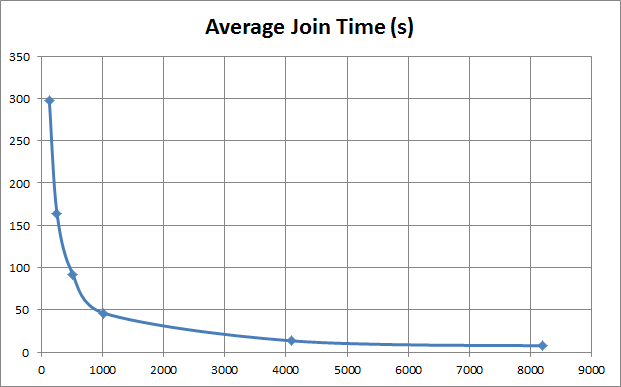
\includegraphics[width=0.48\textwidth]{fig/join_nobatch.png}
            \\
        \end{tabular}
        \caption{Chunk Size vs Average Join Time for Unbatched Interests}
        \label{fig:joinnobatch}
    \end{center}
\end{figure}

\subsection{Experiments with batching} \label{sec:batch}

We ran implemented batching in the following manner: At the start of a video,
all of the chunks required to fill the buffer at requested at once. As these
individual data packets arrive, one new interest is sent out per packet. By
batching the initial requests, we expect to reduce the join time, as well as
guarantee that the buffer is full as much of the time as possible. The effects
of this change are apparent in the results that follow.

%%%%%%%%%%%%%%%%%%%%%%%%%%%%%%%%%%%%%%%%%%%%%%%%%%%%%%%%%%%%%%%%%%%%%%%%%%%%
\subsection{Join Time} \label{sec:join}

\begin{figure}[!htbp]
    \begin{center}
        \begin{tabular}{l}
            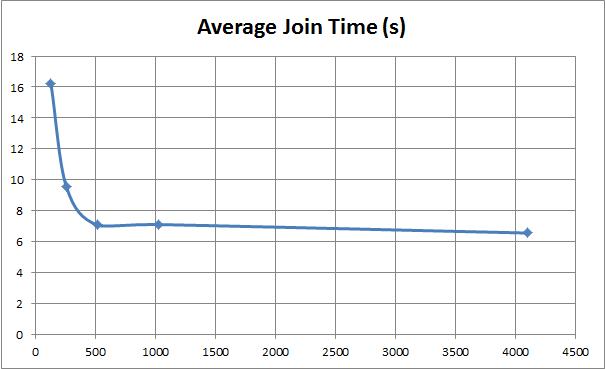
\includegraphics[width=0.48\textwidth]{fig/join.png}
            \\
        \end{tabular}
        \caption{Chunk Size vs Join Time}
        \label{fig:join}
    \end{center}
\end{figure}

We see much more reasonable results for our average join time with batching. The
smaller chunk sizes have a smaller loading time, with the largest value at about
16 seconds for 128 bytes. In the unbatched experiments, as we doubled the chunk
size, the join time was halved. We observe that the join time decreases
exponentially up to 512 bytes, and then is relatively unchanged, at around 7
seconds.

We believe this means that 7 seconds is lower bound for amount of time to download
the buffer size (0.1 of the total video size) for the average video. When the
chunk size is too small or smaller than 512, the router can not keep up with the
quantity of requests even though the bandwidth is available.

%%%%%%%%%%%%%%%%%%%%%%%%%%%%%%%%%%%%%%%%%%%%%%%%%%%%%%%%%%%%%%%%%%%%%%%%%%%
\subsection{Buffering Ratio} \label{sec:bufferingratio}

We excluded a graph of the buffering ratio because we also found it to be 0.0.
We believe this is due to our batching model where chunks are fetched so that
the buffer is full almost all the time. If we had done it differently by for
example, only requesting chunks in batches the size of the buffer every time the
buffer was empty, this value would be non-zero.

%%%%%%%%%%%%%%%%%%%%%%%%%%%%%%%%%%%%%%%%%%%%%%%%%%%%%%%%%%%%%%%%%%%%%%%%%%%%
\subsection{Average PIT size} \label{sec:pit}

\begin{figure}[!htbp]
    \begin{center}
        \begin{tabular}{l}
            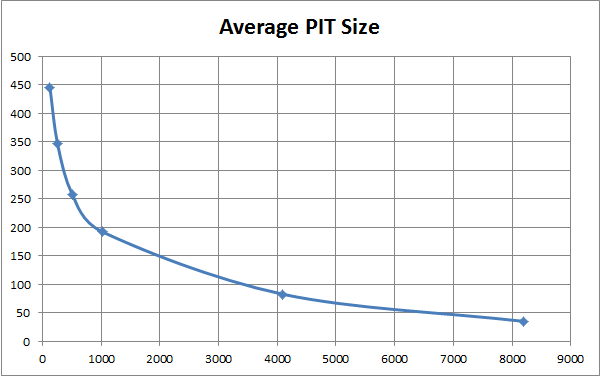
\includegraphics[width=0.48\textwidth]{fig/pit.png}
            \\
        \end{tabular}
        \caption{Chunk Size vs Average PIT Size}
        \label{fig:pit}
    \end{center}
\end{figure}

The PIT size is a measure the load on the routers. If the PIT size is 0, it
implies that the router is able to serve every request as soon as it arrives. If
it greater than 0, it means there are requests that are served with a delay. A
smaller PIT size should correspond to better user experience, therefore.

From the graph, we see that PIT size reduces exponentially, but with a factor
less than 2. Because of how we batch the chunks, we expected that the size of
the PIT should approximately double every time we halve chunk size, because
we always have a $buffer / chunk size$ outstanding requests for every client. It
appears that the router is able to deal with requests for smaller chunk sizes
more effectively, perhaps because there is a higher likelihood of satisfying an
interest with a chunk already in the cache.

%%%%%%%%%%%%%%%%%%%%%%%%%%%%%%%%%%%%%%%%%%%%%%%%%%%%%%%%%%%%%%%%%%%%%%%%%%%%%%%
\subsection{Server Load Reduction} \label{sec:load}

As we expected, server load reduction is greater with smaller chunks, because
the number of cached chunk requests is potentially larger. One interesting point
to note is that the reduction provided by 256 and 512 byte chunks is
approximately the same at 0.1. This may be the range of chunk sizes where the
benefits of increased cache hits on the server load is the greater, or it could
just be an outlier from our dataset.

\begin{figure}[!htbp]
    \begin{center}
        \begin{tabular}{l}
            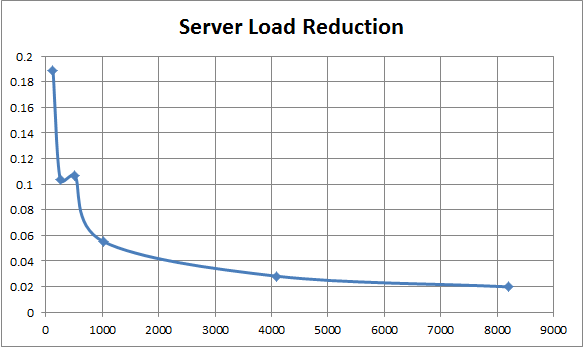
\includegraphics[width=0.48\textwidth]{fig/load.png}
            \\
        \end{tabular}
        \caption{Chunk Size vs Server Load Reduction}
        \label{fig:load}
    \end{center}
\end{figure}

%%%%%%%%%%%%%%%%%%%%%%%%%%%%%%%%%%%%%%%%%%%%%%%%%%%%%%%%%%%%%%%%%%%%%%%%%%%%%%
\subsection{Total View Time} \label{sec:view}

Total view time increases with the size of the chunks, and levels off around
chunk size 4096. The reason that the total view time does not increase linearly
or exponentially is that as the chunk sizes increase indefinitely, the
performance is limited by the bandwidth of the network.


\begin{figure}[!htbp]
    \begin{center}
        \begin{tabular}{l}
            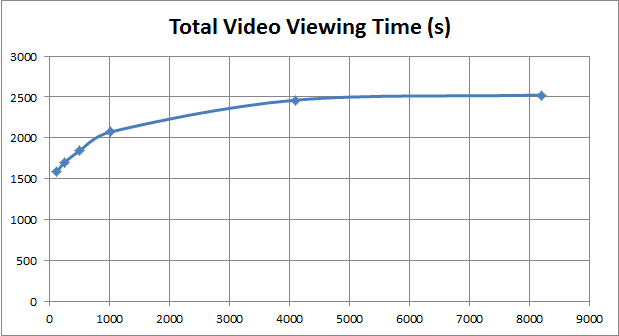
\includegraphics[width=0.48\textwidth]{fig/view.png}
            \\
        \end{tabular}
        \caption{Chunk Size vs Total Viewing Time}
        \label{fig:view}
    \end{center}
\end{figure}


\begin{table*}[ht]
    \centering
    \begin{tabular}{c|cccc}
        \begin{tabular}[c]{@{}c@{}}Chunk Size\\ (bytes)\end{tabular} &
     \begin{tabular}[c]{@{}c@{}}Avg Join Time \\ (s)\end{tabular} &
        \begin{tabular}[c]{@{}c@{}}Avg PIT Size\\ (\# packets)\end{tabular}
        & \begin{tabular}[c]{@{}c@{}}Server Load Reduction\\
            (\%)\end{tabular} & \begin{tabular}[c]{@{}c@{}}Total View Time\\
        (s)\end{tabular} \\ \hline
        128 & 16.20 & 446 & 18.8 & 1584 \\ 256 & 9.55 & 347 & 10.3 &
        1698
        \\ 512 & 7.07 & 257 & 10.7 & 1842 \\ 1024 & 7.10 & 192 & 5.5 &
  2073 \\ 4096 & 6.55 & 82 & 2.8 & 2461 \\ 8192 & 6.47 & 35 & 1.98
               &
        2523
    \end{tabular}
    \caption{Captured metrics for different chunk sizes}
\end{table*}
